\documentclass[a4paper,class=article,border=10pt,tikz]{standalone}

%mypackages
\usepackage{pythontex}
\usepackage{pgfplots}
\usepackage{amsmath}
\usepackage{titlesec}
\usepackage{tikz}
\usetikzlibrary{shapes.geometric}
\usetikzlibrary{positioning}
\usetikzlibrary{snakes,calc,positioning,patterns,angles,quotes,decorations.pathmorphing,decorations.markings}
% \titleformat{<command>}[<shape>]{<format>}{<label>}{<sep>}{<before-code>}[<after-code>]
%\titleformat{\section}{\normalfont\Large\bfseries}{\thesection.}{10pt}{}
% \titlespacing{<command>}{<left>}{<before-sep>}{<after-sep>}
%\titlespacing{\section}{0pt}{14pt}{7pt}

%\titleformat{\subsection}{\normalfont\itshape}{\thesubsection.}{10pt}{}
%\titlespacing{\subsection}{0pt}{12pt}{6pt}
% set font encoding for PDFLaTeX, XeLaTeX, or LuaTeX
\usepackage{ifxetex,ifluatex}
\if\ifxetex T\else\ifluatex T\else F\fi\fi T%
  \usepackage{fontspec}
\else
  \usepackage[T1]{fontenc}
  \usepackage[utf8]{inputenc}
  \usepackage{lmodern}
\fi

\usepackage{hyperref}


\title{Title of Document}
\author{Name of Author}

% Enable SageTeX to run SageMath code right inside this LaTeX file.
% http://doc.sagemath.org/html/en/tutorial/sagetex.html
% \usepackage{sagetex}

% Enable PythonTeX to run Python – https://ctan.org/pkg/pythontex
% \usepackage{pythontex}

\begin{document}


\newpage

% \begin{pycode}
% spring_mount_xshift=-0.5
% \end{pycode}

\begin{pysub}
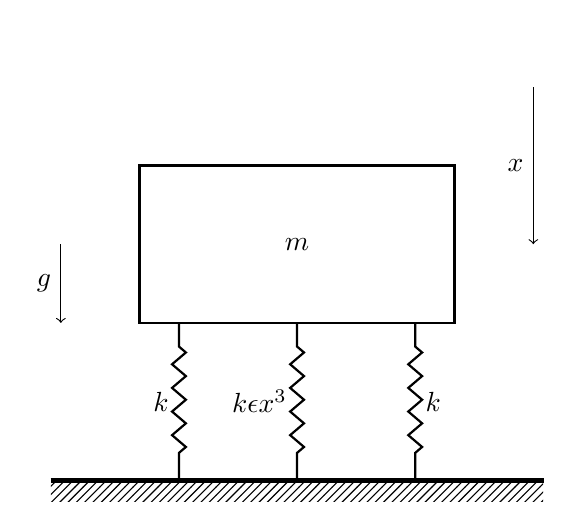
\begin{tikzpicture}[scale=1, transform shape]
 \coordinate (origo) at (0,0);

\tikzstyle{spring}=[thick,decorate,decoration={zigzag,pre length=0.3cm,post length=0.3cm,segment length=0.3cm}]

\tikzstyle{damper}=[thick,decoration={markings,
  mark connection node=dmp,
  mark=at position 0.5 with
  {
    \node (dmp) [thick,inner sep=0pt,transform shape,rotate=-90,minimum width=15pt,minimum height=3pt,draw=none] {};
    \draw [thick] ($(dmp.north east)+(2pt,0)$) -- (dmp.south east) -- (dmp.south west) -- ($(dmp.north west)+(2pt,0)$);
    \draw [thick] ($(dmp.north)+(0,-5pt)$) -- ($(dmp.north)+(0,5pt)$);
  }
}, decorate]

\tikzstyle{ground}=[fill,pattern=north east lines,draw=none,minimum width=0.75cm,minimum height=0.3cm]



   %draw axes
    %\fill[black] (origo) circle (0.05);


    \node (M) [outer sep=0pt,thick,minimum width=3cm, minimum height=1.5cm,yshift=2cm] at (origo) {$$};
    %\node (m1_label) at ($(M)+(0:0.5cm)$) {$m$};

%     \draw [spring] ([xshift=-1cm]origo)  node (k_sup_spring_left){}  -- ([xshift=-1cm]M.south) node[midway,left] {$\frac {k}{2}$};

%         \draw [spring] ([xshift=+1cm]origo) node (k_sup_spring_right){} -- ([xshift=1cm]M.south)   node[midway,right] {$\frac {k}{2}$};

    %\fill [black] (M.center) circle (0.05);

   % \node (beam) [fill=gray,anchor=north,xshift=0cm,yshift=0cm,minimum width=2cm,minimum height=0.05pt] at (origo) {} node[right]{$m_{beam}=0$};

%     \draw [ultra thick] (k_sup_spring_left.west) -- (k_sup_spring_right.east) node[midway] (beam_center) {};



%         \node (road_sur) [fill=black,anchor=north,xshift=0cm,yshift=-2cm,minimum width=2cm,minimum height=0.05cm] at (beam) {};

%beam_center.center

        \draw[spring] ([xshift=-1.5cm,yshift=-1cm]origo.center) -- ++(0,-2cm) node (k_tire_end) {} node[midway,left] {$k$};

        \draw[spring] ([xshift=+1.5cm,yshift=-1cm]origo.center) -- ++(0,-2cm) node (c_tire_end) {} node[midway,right=0.00cm] {$k$};


        \node[draw,outer sep=0pt,thick,fill=white,minimum width=4cm,minimum height=2cm] (M2) at (origo) {};
\draw[spring] ([yshift=-1cm]origo.center) -- ++(0,-2cm) node (k_center_end) {} node[midway,left] {$k\epsilon x^{3}$};

        \node[] at (M2.center) {$m$} ;

    \draw[ultra thick] ([xshift=-1.5cm]k_tire_end.west) -- ([xshift=+1.5cm]c_tire_end.east) node (force_attachment_point) {};

\node (ground1) [ground,rotate=0,anchor=east,xshift=-0cm,yshift=0cm,minimum width=6.25cm,,minimum height=0.2cm] at (force_attachment_point.south) {};

\draw[->] (-3cm,0cm)--++(0,-1cm) node[midway,left] {$g$};
\draw[<-] (3cm,0cm)--++(0,2cm) node[midway,left] {$x$};

\end{tikzpicture}
\end{pysub}




\end{document}
